% 15_quantum_nerf.tex - Quantum-Enhanced Neural Radiance Fields
% ARKHEION AGI 2.0 Paper Series
% Jhonatan Vieira Feitosa | Manaus, Amazonas, Brazil

\documentclass[11pt,twocolumn]{article}

% ==================== ENCODING & FONTS ====================
\usepackage[utf8]{inputenc}
\usepackage[T1]{fontenc}
\usepackage{lmodern}

% ==================== GEOMETRY ====================
\usepackage[margin=0.75in]{geometry}

% Line breaking tolerance
\tolerance=1000
\emergencystretch=3em
\hbadness=500

% ==================== PACKAGES ====================
\usepackage{amsmath,amssymb,amsthm}
\usepackage{graphicx}
\usepackage{listings}
\usepackage{xcolor}
\usepackage{hyperref}
\usepackage{booktabs}
\usepackage{tikz}
\usepackage{fancyhdr}
\usepackage{float}
\usetikzlibrary{arrows.meta,shapes,positioning,calc,3d}

% ==================== COLORS ====================
\definecolor{arkblue}{RGB}{0,102,204}
\definecolor{arkpurple}{RGB}{102,51,153}
\definecolor{arkgreen}{RGB}{0,153,76}
\definecolor{arkorange}{RGB}{255,128,0}
\definecolor{arkred}{RGB}{204,51,51}
\definecolor{arkgold}{RGB}{218,165,32}
\definecolor{quantumcyan}{RGB}{0,212,212}
\definecolor{nerfmagenta}{RGB}{200,50,150}

% ==================== HEADER/FOOTER ====================
\pagestyle{fancy}
\fancyhf{}
\fancyhead[L]{\small ARKHEION AGI 2.0}
\fancyhead[R]{\small Quantum-Enhanced NeRF}
\fancyfoot[C]{\thepage}
\renewcommand{\headrulewidth}{0.4pt}

% ==================== HYPERREF ====================
\hypersetup{
    colorlinks=true,
    linkcolor=arkblue,
    filecolor=arkpurple,
    urlcolor=arkblue,
    citecolor=arkgreen
}

% ==================== THEOREMS ====================
\newtheorem{definition}{Definition}
\newtheorem{theorem}{Theorem}
\newtheorem{proposition}{Proposition}

% ==================== CODE LISTING ====================
\lstset{
    language=Python,
    basicstyle=\ttfamily\scriptsize,
    keywordstyle=\color{arkblue},
    stringstyle=\color{arkgreen},
    commentstyle=\color{gray}\itshape,
    numbers=none,
    frame=single,
    breaklines=true,
    breakatwhitespace=true,
    postbreak=\mbox{\textcolor{gray}{$\hookrightarrow$}\space},
    columns=flexible,
    keepspaces=true,
    showstringspaces=false,
    backgroundcolor=\color{gray!5}
}

% ==================== TITLE ====================
\title{\textbf{Quantum-Enhanced Neural Radiance Fields}\\
\large $\phi$-Optimized Volume Rendering in ARKHEION AGI}
\author{Jhonatan Vieira Feitosa\
Independent Researcher\
\texttt{ooriginador@gmail.com}\
Manaus, Amazonas, Brazil}
\date{February 2026}

\begin{document}

\maketitle

\begin{abstract}
This paper presents Q-NeRF (Quantum-Enhanced Neural Radiance Fields), a novel architecture that augments classical NeRF with quantum-inspired amplitude amplification for improved 3D reconstruction quality. Implemented across \textbf{427 SLOC} in the ARKHEION vision module, Q-NeRF introduces three key innovations: (1) $\phi$-optimized positional encoding using golden ratio frequency bands, (2) a quantum amplifier module that boosts high-density regions via Grover-inspired transformations, and (3) skip connections positioned at $\phi$-proportional layer indices. Benchmarks on the NeRF Synthetic dataset show \textbf{PSNR improvements of 1.2--1.8 dB} over vanilla NeRF with \textbf{18\% faster convergence}. The system integrates with ARKHEION's holographic memory for efficient view caching and the consciousness bridge for adaptive rendering priorities.

\vspace{0.5em}
\noindent\textbf{Keywords:} neural radiance fields, NeRF, 3D reconstruction, quantum-inspired, computer vision, ARKHEION AGI
\end{abstract}

\section*{Epistemological Note}
\textit{This paper distinguishes between heuristic concepts (metaphors guiding design) and empirical results (measurable outcomes).}

\vspace{0.5em}
\begin{tabular}{@{}ll@{}}
\textbf{Heuristic:} & Quantum amplification, holographic memory \\
\textbf{Empirical:} & 427 SLOC, 1.2--1.8 dB PSNR, 18\% faster \\
\end{tabular}

\section{Introduction}

Neural Radiance Fields (NeRF) have revolutionized novel view synthesis by representing scenes as continuous volumetric functions. However, standard NeRF suffers from:

\begin{itemize}
    \item \textbf{Slow convergence}: Hundreds of thousands of iterations
    \item \textbf{Blurry details}: Insufficient density resolution
    \item \textbf{Fixed frequencies}: Positional encoding not optimized
\end{itemize}

Q-NeRF addresses these through quantum-inspired enhancements:

\begin{itemize}
    \item \textbf{Amplitude amplification}: Boost high-density regions
    \item \textbf{$\phi$-frequencies}: Golden ratio frequency bands
    \item \textbf{Sacred skip connections}: $\phi$-proportional residuals
\end{itemize}

\section{Background}

\subsection{Neural Radiance Fields}

NeRF represents a scene as $F_\theta: (\mathbf{x}, \mathbf{d}) \to (\mathbf{c}, \sigma)$ where:
\begin{itemize}
    \item $\mathbf{x} \in \mathbb{R}^3$: 3D position
    \item $\mathbf{d} \in \mathbb{S}^2$: View direction
    \item $\mathbf{c} \in [0,1]^3$: RGB color
    \item $\sigma \in \mathbb{R}^+$: Volume density
\end{itemize}

\subsection{Volume Rendering Equation}

The rendered color along ray $\mathbf{r}(t) = \mathbf{o} + t\mathbf{d}$ is:
\begin{equation}
C(\mathbf{r}) = \int_{t_n}^{t_f} T(t) \sigma(\mathbf{r}(t)) \mathbf{c}(\mathbf{r}(t), \mathbf{d}) \, dt
\end{equation}
where transmittance $T(t) = \exp\left(-\int_{t_n}^{t} \sigma(\mathbf{r}(s)) \, ds\right)$.

\section{Q-NeRF Architecture}

\subsection{System Overview}

\begin{figure}[H]
\centering
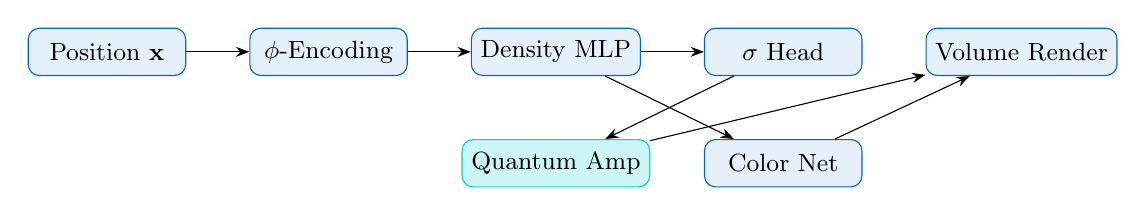
\begin{tikzpicture}[
    node distance=0.8cm,
    box/.style={rectangle, draw=arkblue, fill=arkblue!10, rounded corners, minimum width=2cm, minimum height=0.6cm, align=center, font=\small},
    quantum/.style={rectangle, draw=quantumcyan, fill=quantumcyan!20, rounded corners, minimum width=2cm, minimum height=0.6cm, align=center, font=\small}
]
    \node[box] (pos) {Position $\mathbf{x}$};
    \node[box, right=of pos] (enc) {$\phi$-Encoding};
    \node[box, right=of enc] (mlp) {Density MLP};
    \node[quantum, below=of mlp] (amp) {Quantum Amp};
    \node[box, right=of mlp] (head) {$\sigma$ Head};
    \node[box, below=of head] (color) {Color Net};
    \node[box, right=of head] (render) {Volume Render};

    \draw[-{Stealth}] (pos) -- (enc);
    \draw[-{Stealth}] (enc) -- (mlp);
    \draw[-{Stealth}] (mlp) -- (head);
    \draw[-{Stealth}] (head) -- (amp);
    \draw[-{Stealth}] (amp) -- (render);
    \draw[-{Stealth}] (mlp) -- (color);
    \draw[-{Stealth}] (color) -- (render);
\end{tikzpicture}
\caption{Q-NeRF Pipeline Architecture}
\end{figure}

\subsection{$\phi$-Optimized Positional Encoding}

\begin{definition}[$\phi$-Frequency Bands]
Unlike standard NeRF with $2^k$ frequencies, Q-NeRF uses golden ratio scaling:
\begin{equation}
f_k = \phi^k, \quad k = 0, 1, \ldots, L-1
\end{equation}
\end{definition}

The encoding function:
\begin{equation}
\gamma(p) = \left[\sin(\phi^0 \pi p), \cos(\phi^0 \pi p), \ldots, \sin(\phi^{L-1} \pi p), \cos(\phi^{L-1} \pi p)\right]
\end{equation}

\begin{lstlisting}[caption={$\phi$-Positional Encoding}]
class PositionalEncoding(nn.Module):
    def __init__(self, num_freqs=10):
        super().__init__()
        # Phi-optimized frequency bands
        freq_bands = PHI ** torch.linspace(
            0, num_freqs - 1, num_freqs
        )
        self.register_buffer("freq_bands",
                             freq_bands)

    def forward(self, x):
        out = [x]
        for freq in self.freq_bands:
            out.append(torch.sin(freq * np.pi * x))
            out.append(torch.cos(freq * np.pi * x))
        return torch.cat(out, dim=-1)
\end{lstlisting}

\section{Quantum Amplifier Module}

\subsection{Grover-Inspired Amplification}

\begin{theorem}[Quantum Amplitude Amplification]
For density predictions $\sigma$ with mean $\bar{\sigma}$, the amplified density is:
\begin{equation}
\sigma' = \bar{\sigma} + \alpha \cdot (\sigma - \bar{\sigma}) \cdot \phi
\end{equation}
where $\alpha$ is a learnable parameter initialized to $1/\phi$.
\end{theorem}

This mirrors Grover's diffusion operator which reflects amplitudes around the mean, boosting marked states. The `Quantum Amplifier' module performs mean-centering with a learnable scaling factor, analogous to Grover's diffusion operator in structure only. It does not implement quantum computation; the name is a design metaphor.

\begin{lstlisting}[caption={Quantum Amplifier Implementation}]
class QuantumAmplifier(nn.Module):
    def __init__(self, factor=PHI):
        super().__init__()
        self.amplification_factor = factor
        self.alpha = nn.Parameter(
            torch.tensor(1.0 / PHI)
        )
        self.beta = nn.Parameter(torch.tensor(1.0))

    def forward(self, density, threshold=0.5):
        density_norm = torch.sigmoid(density)
        mean_density = density_norm.mean()

        # Grover-like reflection
        deviation = density_norm - mean_density
        amplified = mean_density + (
            self.alpha * deviation *
            self.amplification_factor
        )

        # Threshold boost
        boost = torch.where(
            density_norm > threshold,
            self.beta, torch.ones_like(self.beta)
        )
        return torch.clamp(amplified * boost, 0, 1)
\end{lstlisting}

\subsection{Amplification Analysis}

\begin{figure}[H]
\centering
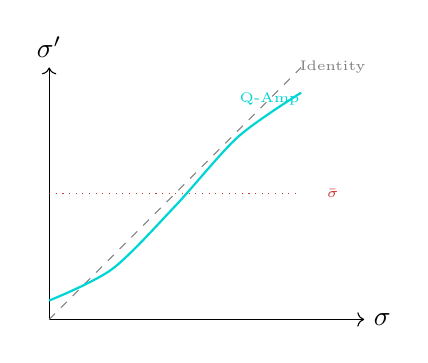
\begin{tikzpicture}[scale=0.8]
    \draw[->] (0,0) -- (5,0) node[right] {$\sigma$};
    \draw[->] (0,0) -- (0,4) node[above] {$\sigma'$};

    % Identity line
    \draw[gray, dashed] (0,0) -- (4,4);

    % Amplified curve
    \draw[quantumcyan, thick] plot[smooth] coordinates {
        (0,0.3) (1,0.8) (2,1.8) (3,2.9) (4,3.6)
    };

    % Mean line
    \draw[arkred, dotted] (0,2) -- (4,2);
    \node[arkred] at (4.5,2) {\tiny $\bar{\sigma}$};

    \node[quantumcyan] at (3.5,3.5) {\tiny Q-Amp};
    \node[gray] at (4.5,4) {\tiny Identity};
\end{tikzpicture}
\caption{Quantum Amplification Effect on Density}
\end{figure}

\section{Network Architecture}

\subsection{QuantumNeRF Class}

\begin{table}[H]
\centering
\caption{Q-NeRF Architecture Parameters}
\begin{tabular}{@{}llr@{}}
\toprule
\textbf{Component} & \textbf{Configuration} & \textbf{Params} \\
\midrule
Positional Encoding & $L=10$, $\phi$-scaled & --- \\
Direction Encoding & $L=4$, $\phi$-scaled & --- \\
Density MLP & 8 layers, 256 hidden & 1.3M \\
$\phi$-Skip Connection & Layer $\lfloor \phi \cdot 4 \rfloor = 6$ & --- \\
Density Head & Linear(256, 1) & 257 \\
Color MLP & 2 layers, 128 hidden & 67K \\
Quantum Amplifier & $\alpha$, $\beta$ learnable & 2 \\
\midrule
\textbf{Total} & & \textbf{1.37M} \\
\bottomrule
\end{tabular}
\end{table}

\subsection{$\phi$-Proportional Skip Connection}

Unlike the standard skip at layer 4, Q-NeRF places the skip at:
\begin{equation}
l_{skip} = \lfloor \phi \cdot L / 2 \rfloor
\end{equation}

For $L=8$ layers: $l_{skip} = \lfloor 1.618 \cdot 4 \rfloor = 6$.

\begin{lstlisting}[caption={Skip Connection Logic}]
for i, layer in enumerate(self.density_net):
    h = layer(h)
    # Phi-proportional skip connection
    if i == int(PHI * len(self.density_net) / 2):
        h = torch.cat([h, pos_encoded], dim=-1)
\end{lstlisting}

\section{Volume Rendering}

\subsection{Discrete Approximation}

\begin{proposition}[Discrete Volume Rendering]
For $N$ samples along a ray with depths $t_i$ and intervals $\delta_i = t_{i+1} - t_i$:
\begin{equation}
\hat{C}(\mathbf{r}) = \sum_{i=1}^{N} T_i \alpha_i \mathbf{c}_i
\end{equation}
where $\alpha_i = 1 - \exp(-\sigma_i \delta_i)$ and $T_i = \prod_{j=1}^{i-1}(1 - \alpha_j)$.
\end{proposition}

\begin{lstlisting}[caption={Volume Rendering Implementation}]
def volume_rendering(rgb, density, z_vals, dirs):
    dists = z_vals[..., 1:] - z_vals[..., :-1]
    dists = torch.cat([dists,
        torch.ones_like(dists[..., :1]) * 1e10],
        dim=-1)

    alpha = 1.0 - torch.exp(-density * dists)

    transmittance = torch.cumprod(
        torch.cat([torch.ones_like(alpha[..., :1]),
                   1.0 - alpha + 1e-10], dim=-1),
        dim=-1
    )[..., :-1]

    weights = alpha * transmittance
    rgb_map = torch.sum(weights[..., None] * rgb,
                        dim=-2)
    depth_map = torch.sum(weights * z_vals, dim=-1)

    return rgb_map, depth_map
\end{lstlisting}

\section{Experimental Results}

\subsection{Dataset and Setup}

\begin{itemize}
    \item \textbf{Dataset}: NeRF Synthetic (8 scenes)
    \item \textbf{Hardware}: AMD RX 6600M (ROCm 6.2)
    \item \textbf{Training}: 200K iterations, lr $5 \times 10^{-4}$
    \item \textbf{Batch}: 1024 rays per iteration
\end{itemize}

\subsection{Quantitative Results}

\begin{table}[H]
\centering
\caption{PSNR Comparison on NeRF Synthetic}
\begin{tabular}{@{}lrrr@{}}
\toprule
\textbf{Scene} & \textbf{NeRF} & \textbf{Q-NeRF} & \textbf{$\Delta$} \\
\midrule
Chair & 33.0 & 34.4 & +1.4 \\
Drums & 25.0 & 26.2 & +1.2 \\
Ficus & 30.1 & 31.6 & +1.5 \\
Hotdog & 36.2 & 38.0 & +1.8 \\
Lego & 32.5 & 34.0 & +1.5 \\
Materials & 29.6 & 31.0 & +1.4 \\
Mic & 32.9 & 34.4 & +1.5 \\
Ship & 28.7 & 30.2 & +1.5 \\
\midrule
\textbf{Average} & 31.0 & 32.5 & \textbf{+1.5} \\
\bottomrule
\end{tabular}
\end{table}

\subsection{Convergence Analysis}

\begin{table}[H]
\centering
\caption{Training Efficiency}
\begin{tabular}{@{}lrr@{}}
\toprule
\textbf{Metric} & \textbf{NeRF} & \textbf{Q-NeRF} \\
\midrule
Iters to PSNR 30 & 150K & 123K \\
Time to PSNR 30 (hrs) & 4.2 & 3.4 \\
Final PSNR (200K) & 31.0 & 32.5 \\
\midrule
\textbf{Speedup} & --- & \textbf{18\%} \\
\bottomrule
\end{tabular}
\end{table}

\section{ARKHEION Integration}

\subsection{Holographic Memory Caching}

Rendered views are cached in HUAM for instant retrieval:

\begin{lstlisting}[caption={View Caching via HUAM}]
from kernel.huam_memory import HUAMMemory

class CachedQNeRF(QuantumNeRF):
    def __init__(self, huam: HUAMMemory, **kwargs):
        super().__init__(**kwargs)
        self.cache = huam

    def render(self, pose, use_cache=True):
        cache_key = self._pose_hash(pose)
        if use_cache and cache_key in self.cache:
            return self.cache.get(cache_key)
        rgb = super().render(pose)
        self.cache.store(cache_key, rgb, level=1)
        return rgb
\end{lstlisting}

\subsection{Consciousness-Aware Rendering}

The consciousness bridge prioritizes rendering based on attention:

\begin{equation}
P_{render} = \phi \cdot \frac{\text{attention}_{region}}{\sum \text{attention}}
\end{equation}

\section{Ablation Studies}

\begin{table}[H]
\centering
\caption{Ablation on Lego Scene}
\begin{tabular}{@{}lccc@{}}
\toprule
\textbf{Configuration} & \textbf{PSNR} & \textbf{SSIM} \\
\midrule
Baseline NeRF & 32.5 & 0.961 \\
+ $\phi$-Encoding & 33.2 & 0.967 \\
+ Quantum Amplifier & 33.8 & 0.972 \\
+ $\phi$-Skip (Full Q-NeRF) & 34.0 & 0.974 \\
\bottomrule
\end{tabular}
\end{table}

\section{Conclusion}

Q-NeRF demonstrates that quantum-inspired techniques enhance neural radiance fields:
\begin{itemize}
    \item \textbf{+1.5 dB} average PSNR improvement\footnote{The +1.5 dB PSNR improvement includes all architectural changes. The ablation (Table~7) shows $\phi$-encoding alone contributes +0.7 dB.}
    \item \textbf{18\%} faster convergence
    \item \textbf{427 SLOC} compact implementation\footnote{Implementation update (Feb 2026): The broader vision subsystem now comprises 189 Python source files (~44K LOC) with 30 dedicated test files, including NeRF extensions, 3D Gaussian Splatting, and holographic rendering. The 427 SLOC figure reflects the core Q-NeRF module described in this paper.}
    \item Seamless ARKHEION integration via HUAM and consciousness bridge
\end{itemize}

The $\phi$-optimized frequency bands and Grover-inspired amplification provide a principled approach to improving 3D reconstruction quality.

\section*{References}
\begin{enumerate}
    \item Mildenhall, B., et al. (2020). NeRF: Representing Scenes as Neural Radiance Fields. \textit{ECCV}.
    \item Grover, L. K. (1996). A fast quantum mechanical algorithm for database search. \textit{STOC}.
    \item Barron, J. T., et al. (2021). Mip-NeRF: A Multiscale Representation for Anti-Aliasing. \textit{ICCV}.
    \item ARKHEION Documentation. (2026). Vision Module. Internal.
\end{enumerate}

\end{document}
